
Let the given points in the angular axis be
\begin{equation}
\myvec{x_1\\y_1} = \ \myvec{4 \\5} \ ; \ \myvec{x_2\\y_2} \ = \myvec{7\\ 6}\label{2/solution/2/11.0.1}
\end{equation}
From    Fig. \ref{2/solution/2/1Fig1: Points plotted in Python},
the corresponding points in the rectangular axis are
\begin{align}
x_3 = x_1+y_1\cos 60\degree\\
y_3 = y_1\cos 30\degree
% \end{align}
% In order to convert to rectangular coordinate system, the y-axis should be rotated by $30\degree$ in anti-clockwise.
% Transformed coordinates of \myvec{x_1\\y_1} \& \myvec{x_2\\y_2} be \myvec{x_3\\y_3} \& \myvec{x_4\\y_4} respectively.
% \begin{equation}
\implies \myvec{x_3\\y_3} = \myvec{1 \ \cos{60\degree} \\ 0 \  \cos{30\degree}} \myvec{x_1\\y_1}\label{2/solution/2/1eq:1.0.2}   
\end{align}
% \end{equation}
Similarly,\\
\begin{align}
    \myvec{x_4\\y_4} = \myvec{1 \ \cos{60\degree} \\ 0 \  \cos{30\degree}} \myvec{x_2\\y_2}\label{2/solution/2/1eq:1.0.3}
\end{align}
    
% $x_4$ = O$X_2$ + $X_2$$X_4$ = $x_2$+$y_2$\cos{60\degree$$ \\
% $y_4$ = O$Y_2$$\cos{30\degree$$  =\ $y_2$$\cos{30\degree$\\
% \begin{equation}
% \end{equation}
In general, the rectangular coordinates can be express in terms of the angular coordinates through the 
linear transformation
\begin{align}
    \vec{x}_r &= \vec{P}\vec{x}, \\
    \text{where, }
vec{P}&= \myvec{1   &  \cos \theta \\ 0 & \sin \theta} 
\end{align}
Thus, the distance between two points $\vec{x}_1, \vec{x}_2$ in the angular axis  is given by
\begin{align}
    \norm{\vec{P}\brak{\vec{x}_1-\vec{x}_2}} &= \sqrt{\brak{\vec{x}_1-\vec{x}_2}^\top\vec{P}^\top \vec{P}\brak{\vec{x}_1-\vec{x}_2}} \\
    &= \sqrt{13}
\end{align}


% Substituting \eqref{2/solution/2/11.0.1} in \eqref{2/solution/2/1eq:1.0.2} \& \eqref{2/solution/2/1eq:1.0.3}
%  \begin{equation}
%   \myvec{x_3\\y_3} = \myvec{\frac{13}{2}\\\frac{5\sqrt{3}}{2}};\ \myvec{x_4\\y_4} = \myvec{10\\3\sqrt{3}}\label{2/solution/2/1eq:1.0.5}    
%  \end{equation}
% The distance between points is a norm of the distance vector,\\ \norm{\myvec{x_3\\y_3} - \myvec{x_4\\y_4}} = \norm{\myvec{10\\3\sqrt{3}} - \myvec{\frac{13}{2}\\\frac{5\sqrt{3}}{2}}} = 
%  $ \  \sqrt{13} \  units$\\ \\
%  The distance, d can be measured in angular axes directly by following equation,
%  \begin{align}
%  d = \sqrt{{\norm{\myvec{x_2\\y_2} - \myvec{x_1\\y_1}}}^2 +2\myvec{x_2-x_1\\0}^\top \myvec{y_2-y_1\\0}\cos{\theta}}\\ 
% d = \sqrt{{\norm{\myvec{7\\6} - \myvec{4\\5}}}^2 +2\myvec{3&0} \myvec{1\\0}\cos{60\degree}} 
% \end{align}
% \begin{align}
% d = \sqrt{13} \ units    
%  \end{align}
%  \\
% Above results shows that the distance remains constant between the points irrespective of coordinate system and by \eqref{2/solution/2/11.0.1} \& \eqref{2/solution/2/1eq:1.0.5} only the position vector of the point changes with the transformation of coordinate system\\ \\ 
\begin{figure}[!ht]
	\centering
	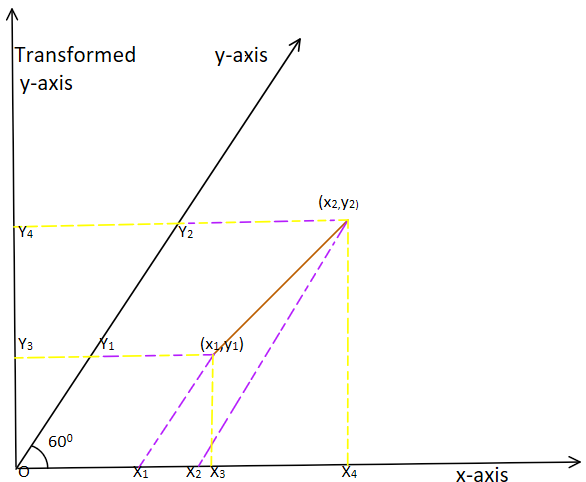
\includegraphics[width=\columnwidth]{2/solution/2/1/fig1.png}
	\caption{Points defined on angular \& rectangular axes}
    \label{2/solution/2/1Fig1: Points plotted in Python}

	\end{figure}
	
% \counterwithin{figure}{section}
% \begin{figure}[!ht]
%     \centering
%     \includegraphics[width=\columnwidth]{2/solution/2/1download.png}
%     \caption{Points plotted in Python}
%     \label{2/solution/2/1Fig2: Points plotted in Python}
% \end{figure}
